\documentclass[a4paper]{article}
\usepackage{WUSTReport}
\usepackage{amsmath}
\usepackage[polish,main=english]{babel}
\usepackage{indentfirst}
\usepackage{natbib}
\usepackage{listings}
\usepackage{matlab-prettifier}
\usepackage{systeme}
\usepackage{todonotes}

\title{Numerical Methods and Optimization Report 1:
  Direct Methods for Solving Linear Systems}
\author{Kinga Otczyk 268473\\Sergiusz Warga 230757}
\date{2025-03-21}
\reporttutor{dr hab. inż. Rafał Zdunek}
\reportgroup{Friday 13:15}

\begin{document}

\maketitle
\tableofcontents
\pagebreak

\section{Problems}
\subsection{Problem 1}%
\label{sec:problem_1}
Find the solution that best approximates the system of inconsistent linear equations:
\begin{tasks}(3)
  \task $\systeme{3x_1-x_2=4,x_1+2x_2=0,2x_1+x_2=1}$
  \task $\systeme{3x_1+x_2+x_3=6,
  2x_1+3x_2-x_3=1,
  2x_1-x_2+x_3=0,
  3x_1-3x_2+3x_3=8}$
  \task $\systeme{x_1+x_2-x_3=5,
  2x_1-x_2+6x_3=1,
  -x_1+4x_2+x_3=0,
  3x_1+2x_2-x_3=6}$
\end{tasks}
%%%%%%%%%%%%%%%%%%%%%%%%%%%%%%%%%%%%%%%%%%%%%%%%%%%%%%%%%%%%%%%%%%%%%%%%%%%%%%%
\subsubsection*{Mathematics}
%%%%%%%%%%%%%%%%%%%%%%%%%%%%%%%%%%%%%%%%%%%%%%%%%%%%%%%%%%%%%%%%%%%%%%%%%%%%%%%
The system of inconsistent linear equations comprises linearly independent equations,
whose number is greater than the number of unknown variables.
Such a system may be expressed in the form:
\begin{equation*}
  \matr{Ax}=\matr{b}, \quad \text{where} \quad
  \matr{A}\in\mathfrak{R}^{m\times{}n}, \quad
  \matr{b}\in\mathfrak{R}^m, \quad
  \matr{x}\in\mathfrak{R}^n, \quad \text{and} \quad m\geq{}n
\end{equation*}
and has no solution. We may attempt to find the best approximate solution to such a
system by solving the minimization problem:
\begin{equation*}
  \min_{\matr{x}}{\left\lVert\matr{b}-\matr{A}\matr{x}\right\rVert}_2
\end{equation*}
For such a system, an associated system of \textit{normal equations} is defined to be:
\begin{equation}
  \matr{A}^T\matr{Ax}=\matr{A}^T\matr{b}
\end{equation}
which is always consistent.
The solution has the form:
\begin{equation}
  \label{eq:normal_approximation}
  \matr{x}=\left(\matr{A}^T\matr{A}\right)^{-1}\matr{A}^T\matr{b}
\end{equation}
%%%%%%%%%%%%%%%%%%%%%%%%%%%%%%%%%%%%%%%%%%%%%%%%%%%%%%%%%%%%%%%%%%%%%%%%%%%%%%%
\subsubsection*{Solution}
%%%%%%%%%%%%%%%%%%%%%%%%%%%%%%%%%%%%%%%%%%%%%%%%%%%%%%%%%%%%%%%%%%%%%%%%%%%%%%%
The solutions to all the systems of linear equations above may be easily approximated
with the \MATLAB{} function implementing~\eqref{eq:normal_approximation}:
\lstinputlisting[style=Matlab-editor]{problems/normal_approximation.m}
Then, the solution may be verified with \lstinline[style=Matlab-editor]{x - A\b}:
\lstinputlisting[style=Matlab-editor]{problems/Problem_1.m}

\subsection{Problem 2}%
\label{sec:problem_2}
Compute the largest and the smallest eigenvalue to the following matrix, using the
scaled power algorithm and the shifted inverse power algorithm, respectively:
\begin{equation*}
    \matr{A} = 
    \begin{bmatrix}
        4 & 2 & 0 & 0 \\
        1 & 4 & 1 & 0 \\
        0 & 1 & 4 & 1 \\
        0 & 0 & 2 & 4
    \end{bmatrix}
\end{equation*}
%%%%%%%%%%%%%%%%%%%%%%%%%%%%%%%%%%%%%%%%%%%%%%%%%%%%%%%%%%%%%%%%%%%%%%%%%%%%%%%
\subsubsection*{Mathematics}
%%%%%%%%%%%%%%%%%%%%%%%%%%%%%%%%%%%%%%%%%%%%%%%%%%%%%%%%%%%%%%%%%%%%%%%%%%%%%%%
Basing on information included in ~\cite{Zdunek}, methods that allow for finding eigenpairs are \textit{Power method} 
(in sources such as refered as \textit{Power iteration}) and \textit{shifted inverse power method}, (Also known as \textit{inverse iteration}\cite{Demmel}).\\
\\
Power iteration allows for quick and easy computation of dominant eigenvalue and coresponding eigenvector $(\lambda_1, x_1)$ of diagonalizable matrix 
\textbf{A}$\in \mathfrak{R}^{n_xn}$ where eigenvalues are in following sequence $|\lambda_1| > |\lambda_2| > ... > |\lambda_n|$.
Initial condition for power method requires random vector that is approximation of dominant eigenvector, which is symbolized as $\xi_0$. Vector generated as such is then immediately which is also normalized in the same step 
\begin{equation*}
    \xi_0 = \frac{\xi_0}{||\xi_0||_2} 
\end{equation*}
This step is done to prevent problems with approximation, underflow, overflows and hold the convergence criterion, it helps at making successive approximations of the eigenvector where normalization helps the randomly generated vector focus on the direction rather than magnitude, reducing algorithm runtime allowing for faster honing to direction of dominant vector.\\
Power iteration as name suggests is iterative technique which computes the result in each loop iteration.
Update formula is similar to initial vector normalization taking into calculation base matrix on which we are trying to define dominant eigenvector
\begin{equation*}
    \xi_k = \frac{A \xi_{k-1}}{||A \xi_{k-1}||_2}
\end{equation*}
Each loop step hones closer to the direction of dominant eigenvector. Because of iterative nature of algorithm, we can break out of the loop after certain amount of steps or after we reach threshold convergence rate $\epsilon$, which is calculated by normalizing the difference between $\xi_k$ and $\xi_{k-1}$.
\begin{equation*}
    ||\xi_k - \xi_{k-1}|| < \epsilon
\end{equation*}
As a final step of power method we need to extract our dominant eigenpair. 
Method for obtaining approximation of our dominant eigenvector is taking last $\xi_k$.\\
Obtaining eigenvalue is bit more complex
\begin{equation*}
    \lambda_1 \approx \xi_k^T A \xi_k 
\end{equation*}
\\
One of biggest disadvantages of Power method is that it can only determine dominant eigenpair, for finding other eigenpairs we need to use more complex variation which is Inverse iteration.
Inverse power method allows for finding any eigenpair, by variable $\sigma$ also known as shift\cite{Demmel}.
Specified $\sigma$ value allows us to converge to the closest eigenvalue to shift rather than only $\lambda_1$. Further steps in loop deviate slightly from Power method, steps that update our next $\xi_k$, we no longer multiply A by previous $\xi_{i-1}$. This calculation also takes in consideration shift modifying formula for next $\xi$ as such:
\begin{equation*}
    \begin{matrix}
        y = (A - \sigma I)^-1 \xi_{i-1}\\
        \xi_i = \frac{y}{||y||_2}
    \end{matrix}
\end{equation*}
Further steps stay consistent with Power method.

\subsubsection*{Solution}
Script that plots and displays results from both methods used accordingly to it's specific task:
\lstinputlisting[style=Matlab-editor]{problems/Codes/Problem_2/main.m}

Running MATLAB script yields such results:
\lstinputlisting[style=Matlab-editor]{problems/Results/Problem_2.m}

\begin{figure}[H]
    \centering
    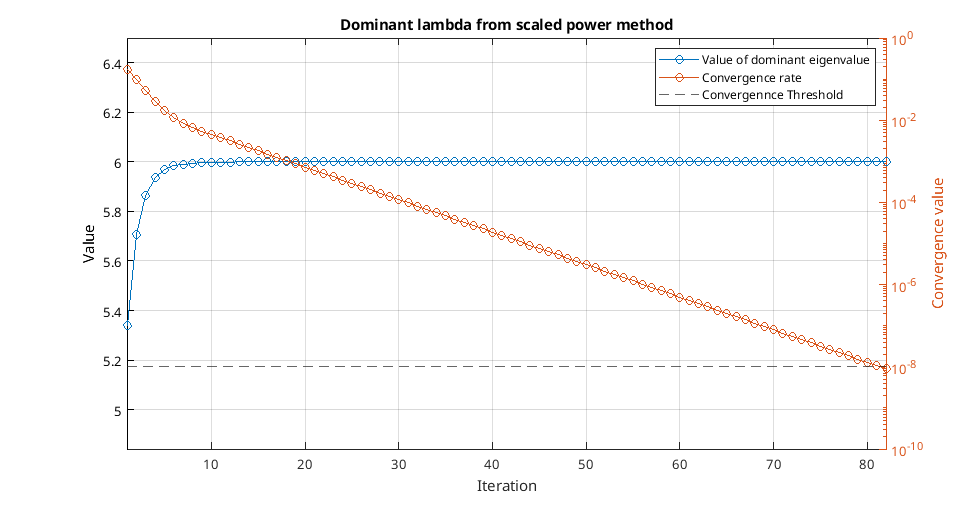
\includegraphics[width=1\textwidth]{problems/Figures/Problem2ScaledPowerMethod.png}
    \caption{Eigenvalue approximation and convergence rate over each iteration of power method.}
    \label{fig:Power}
\end{figure}

\begin{figure}[H]
    \centering
    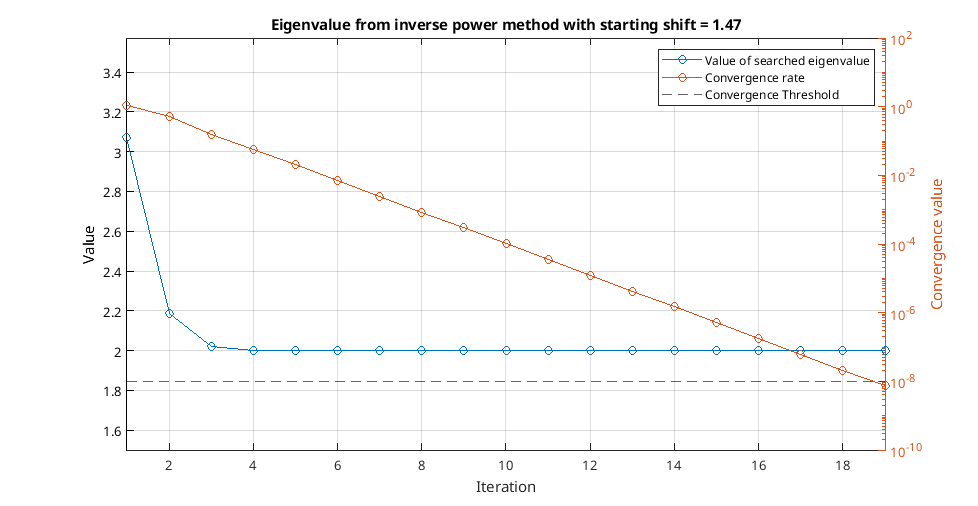
\includegraphics[width=1\textwidth]{problems/Figures/Problem2InversePowerMethod.png}
    \caption{Eigenvalue approximation and convergence rate over each iteration of inverse power method.}
    \label{fig:Inverse}
\end{figure}
% https://tobydriscoll.net/fnc-julia/krylov/inviter.html
% https://www.netlib.org/utk/people/JackDongarra/etemplates/node96.html

\subsection{Problem 3}%
\label{sec:problem_3}
The yield $y$ of wheat in quintals per hectare appears to be a linear function of the
number of days $x_1$ of sunshine, the number of centimeters $x_2$ of rainfall, and the
number of kilograms $x_3$ of fertilizer per hectare. Find the best fit to the data in
the table with an equation in the form: $y=a_0+a_1x_1+a_2x_2+a_3x_3$.

\begin{center}
\begin{tabular}{|c|c|c|c|}
  \hline
  $y$ & $x_1$ & $x_2$ & $x_3$ \\
  \hline
  28 & 50 & 18 & 10 \\
  \hline
  30 & 40 & 20 & 16 \\
  \hline
  21 & 35 & 14 & 10 \\
  \hline
  23 & 40 & 12 & 12 \\
  \hline
  23 & 30 & 16 & 14 \\
  \hline
\end{tabular}
\end{center}

%%%%%%%%%%%%%%%%%%%%%%%%%%%%%%%%%%%%%%%%%%%%%%%%%%%%%%%%%%%%%%%%%%%%%%%%%%%%%%%
\subsubsection*{Mathematics}
%%%%%%%%%%%%%%%%%%%%%%%%%%%%%%%%%%%%%%%%%%%%%%%%%%%%%%%%%%%%%%%%%%%%%%%%%%%%%%%
\todo[inline]{Develop math description}
%%%%%%%%%%%%%%%%%%%%%%%%%%%%%%%%%%%%%%%%%%%%%%%%%%%%%%%%%%%%%%%%%%%%%%%%%%%%%%%
\subsubsection*{Solution}
%%%%%%%%%%%%%%%%%%%%%%%%%%%%%%%%%%%%%%%%%%%%%%%%%%%%%%%%%%%%%%%%%%%%%%%%%%%%%%%

\subsection{Problem 4}%
\label{sec:problem_4}
Using least squares find the ``best'' straight-line fit and the error estimates for the
slope and intercept of that line for the following set of data:
\begin{center}
  \begin{tabular}{|c|c|c|c|c|c|c|c|c|}
    \hline
    $x_i$ & 1 & 2 & 3 & 4 & 5 & 6 & 7 & 8 \\
    \hline
    $y_i$ & 1.5 & 2.0 & 2.8 & 4.1 & 4.9 & 6.3 & 5.0 & 11.5 \\
    \hline
  \end{tabular}
\end{center}
%%%%%%%%%%%%%%%%%%%%%%%%%%%%%%%%%%%%%%%%%%%%%%%%%%%%%%%%%%%%%%%%%%%%%%%%%%%%%%%
\subsubsection*{Mathematics}
%%%%%%%%%%%%%%%%%%%%%%%%%%%%%%%%%%%%%%%%%%%%%%%%%%%%%%%%%%%%%%%%%%%%%%%%%%%%%%%
We want to fit the data above to the function in the form $y = a_0 + a_1x$.
We may proceed with this problem just as in the previous ones.
\todo[inline]{Write something about the linear regression}
%%%%%%%%%%%%%%%%%%%%%%%%%%%%%%%%%%%%%%%%%%%%%%%%%%%%%%%%%%%%%%%%%%%%%%%%%%%%%%%
\subsubsection*{Solution}
%%%%%%%%%%%%%%%%%%%%%%%%%%%%%%%%%%%%%%%%%%%%%%%%%%%%%%%%%%%%%%%%%%%%%%%%%%%%%%%

\subsection{Problem 5}
Find $\mathbf{A^{-1}}$ to:

\begin{equation*}
    \matr{A} = 
    \begin{bmatrix}
        2 & 1 & 2 \\
        1 & 2 & 3 \\
        4 & 1 & 2 
    \end{bmatrix}
\end{equation*}

solving the system $\mathbf{AX=I_{3}}$.

\subsubsection*{Solution}
\lstinputlisting[style=Matlab-editor]{problems/Problem_5.m}
which judges well our algorithms.

\subsection{Problem 6}

Apply the LU factorization to the matrix
\begin{equation*}
    \matr{A} = 
    \begin{bmatrix}
        \phantom{-}1 & 2 & 3 & 4 \\
        -1 & 1 & 2 & 1 \\
        \phantom{-}0 & 2 & 1 & 3 \\
        \phantom{-}0 & 0 & 1 & 1
    \end{bmatrix}
\end{equation*}
Then calculate $\det(\matr{A})$ using the matrix $\matr{U}$. Finally solve $\matr{A}\matr{x}=\matr{b}$ for $\matr{b}=[1\dots1]^T$.
\subsubsection*{Mathematics}
The LU Factorization decomposes matrix $\matr{A}$ into an upper triangular matrix $\matr{U}$ and unit lower triangular matrix $\matr{L}$, so that
\begin{equation*}
    \matr{A} = \matr{L}\matr{U}
\end{equation*}
Using the property of a determinant and a fact, that $\det(\matr{L}) = 1$ one can calculate $\det(\matr{A})$ as
\begin{equation*}
    \det(\matr{A}) = \det(\matr{L}\matr{U}) = \det(\matr{L}) \cdot \det(\matr{U}) = \det(\matr{U}) = u_{11}\cdots u_{nn}
\end{equation*}
\subsubsection*{Solution}
A glance at the matrix $\matr{A}$ tells us that it is not strictly diagonally dominant, so a pivoting algorithm should be used.
%\footnote{$\matr{A}\in\mathbb{R}^{n\times n}$ is \textit{strictly diagonally dominant} if $|a_{ii}|>\sum_{j=1 j i}^n|a_{ij}|$}
\lstinputlisting[style=Matlab-editor]{problems/Problem_6.m}

\subsection{Problem 9}
Let  $\mathbf{A}$  be  the  Pascal  matrix  of  order  100  (\textit{pascal}  function  in Matlab).  Check  whether the matrix is positive definite. If so, apply the Cholesky factorization and give interpretation of the obtained factor.


\subsection{Problem 10}
Transform  the  following  matrix  to  the  RREF,  determine $rank(\mathbf{A})$ and  identify  the columns corresponding to the basic and free variables. 
\begin{equation*}
    \matr{A} = 
    \begin{bmatrix}
    1 & 2 & 2 & 3 & 1 \\
    2 & 4 & 4 & 6 & 2 \\
    3 & 6 & 6 & 9 & 6 \\
    1 & 2 & 4 & 5 & 3 
    \end{bmatrix}
\end{equation*}

Check whether the symmetric matrix $\mathbf{A}$ is positive-definite. If so, apply the Cholesky factorization. Then, compute its inverse.

\subsubsection*{Solution}

\begin{equation*}
    \begin{split}
    \begin{bmatrix}
    1 & 2 & 2 & 3 & 1 \\
    2 & 4 & 4 & 6 & 2 \\
    3 & 6 & 6 & 9 & 6 \\
    1 & 2 & 4 & 5 & 3 
    \end{bmatrix}
    \xrightarrow{\substack{R_2 - 2R_1 \\ R_3 - 3R_1 \\ R_4 - R_1}}
    \begin{bmatrix}
    1 & 2 & 2 & 3 & 1 \\
    0 & 0 & 0 & 0 & 0 \\
    0 & 0 & 0 & 0 & 3 \\
    0 & 0 & 2 & 2 & 2
    \end{bmatrix}
    \xrightarrow{pivot}
    \begin{bmatrix}
    1 & 2 & 2 & 3 & 1 \\
    0 & 0 & 2 & 2 & 2 \\
    0 & 0 & 0 & 0 & 3 \\
    0 & 0 & 0 & 0 & 0
    \end{bmatrix}
    \\
    \xrightarrow{\substack{R_2 / 2 \\ R_3 / 3}}
    \begin{bmatrix}
    1 & 2 & 2 & 3 & 1 \\
    0 & 0 & 1 & 1 & 1 \\
    0 & 0 & 0 & 0 & 1 \\
    0 & 0 & 0 & 0 & 0
    \end{bmatrix}
    \xrightarrow{\substack{R_1 - R_3 \\ R_2 - R_3}}
    \begin{bmatrix}
    1 & 2 & 2 & 3 & 0 \\
    0 & 0 & 1 & 1 & 0 \\
    0 & 0 & 0 & 0 & 1 \\
    0 & 0 & 0 & 0 & 0
    \end{bmatrix}
    \end{split}
\end{equation*}

Rank of the given matrix is equal to 3.



\clearpage

\section{Algorithms}
\subsection{Back substitution}%
\label{algorithm:back_substitution}
\lstinputlisting[style=Matlab-editor, breaklines=false]{algorithms/back_substitution.m}
\subsection{Gaussian elimination}%
\label{algorithm:gaussian_elimination}
\lstinputlisting[style=Matlab-editor, breaklines=false]{algorithms/gaussian_elimination.m}
\subsection{Gaussian elimination with partial pivoting}
\label{algorithm:gaussian_elimination_with_partial_pivoting}
\subsection{Algorithm~2: Gaussian elimination with Complete Pivoting}%
\label{algorithm:2}
\lstinputlisting[style=Matlab-editor, breaklines=false]{algorithms/Alg2.m}
\subsection{Algorithm~3: Forward Substitution}%
\label{algorithm:3}
\lstinputlisting[style=Matlab-editor, breaklines=false]{algorithms/Alg3.m}
\subsection{Algorithm~5: The Gauss-Jordan elimination algorithm}%
\label{algorithm:5}
\lstinputlisting[style=Matlab-editor, breaklines=false]{algorithms/Alg5.m}
\subsection{Algorithm~6: The RREF algorithm}%
\label{algorithm:6}
\lstinputlisting[style=Matlab-editor, breaklines=false]{algorithms/Alg6_RREF.m}
% \subsection{Algorithm 7 -- The LU  factorization without pivoting}\label{algorithm:7}
% \lstinputlisting[style=Matlab-editor]{algorithms/Alg7.m}
% \subsection{Algorithm 8 -- The LU  factorization with partial pivoting}\label{algorithm:8}
% \lstinputlisting[style=Matlab-editor]{algorithms/Alg8.m}
% \subsection{Algorithm 9 -- A family of the Cholesky  factorization  algorithms}\label{algorithm:9}
% \lstinputlisting[style=Matlab-editor]{algorithms/Alg9.m}
% \stepcounter{subsection}
% \subsection{Algorithm 10 -- The Cholesky factorization}\label{algorithm:10}
% \lstinputlisting[style=Matlab-editor]{algorithms/Alg10.m}

%%%%%%%%%%%%%%%%%%%
%% BIBLIOGRAPHY %%%
%%%%%%%%%%%%%%%%%%%

\clearpage

\nocite{Zdunek, GoluVanl96, Meyer}
\bibliographystyle{alpha}
\bibliography{bibliography}

\end{document}
